\documentclass[a4paper, 15pt,titlepage]{article}

\usepackage{Paquetes}
\usepackage{float}

\graphicspath{{./Unidad 1/Imagenes}}

\begin{document}
	%para mi en este principal haces la portada y vas incluyendo cada desarrollo de cada unidad
	%tambien se puede hacer en este el encabezado y pie de pagina pero nose como andaria voy a probar
	\begin{titlepage}
		\begin{center}		
			{\huge \textbf{Universidad Tecnológica Nacional}}\\
			{\huge \textbf{Facultad Regional Reconquista}}
			
			\vspace{1cm}
			
			
\includegraphics[width=0.40\linewidth]{UTNLOGO}\\
			
			\vspace{1cm}
			
			{\huge\textbf{Ingeniería Electromecánica}}
			
			\vspace{1cm}
			
			{\textbf{Año}: 4°} \hspace{5cm}  {Diseño Curricular: 2004 - Ordenanza N°1029 }
			
			\vspace{1cm}
			
			{{\LARGE  \textbf{Mecánica de los fluidos y máquinas fluido dinámicas}}}
			\vspace{1cm}
			
			{\LARGE \textbf{Resumen de teoria}}
			
		\end{center}
		
		\begin{flushleft}
			\Large
			\textbf{Integrantes:}\\
			\vspace{5mm}
			\hspace{3cm}Faulkner Melani\\
			\vspace{5mm}
			\hspace{3cm}Franzoi Valentin\\
			\vspace{5mm}
			\hspace{3cm}Guardiani Franco\\
			\vspace{5mm}
			\hspace{3cm}Polo Daiana
			
		\end{flushleft}
	\end{titlepage}
	
	%\usepackage{Paquetes}

\fancyfoot{}
\rfoot{{\small Pág. \thepage}}
\lfoot{{\footnotesize \textbf{Alumnos:} Los mas capos}}
\fancyhead{}
\lhead{{\footnotesize Mecánica de fluidos \\ \textit{UTN - Facultad Regional Reconquista}}}
\rhead{{\footnotesize \textsc{Unidad 1: Propiedades de fluidos}}}
\setlength{\headsep}{1.2cm}

\setlength{\parindent}{0pt}%para sacar la sangría

\section{Unidad 1: Conceptos fundamentales}
\subsection{Definición de fluido y continuo}
Un fluido es aquel que se deforma continuamente cuando se somete a esfuerzos cortantes, por mas mínimos que estos resulten.
\begin{figure}[h]
	\centering
	\begin{subfigure}[b]{0.45\linewidth}
		
\includegraphics[width= .5\linewidth]{cortante1}
	\end{subfigure}
	\begin{subfigure}[b]{0.45\linewidth}
		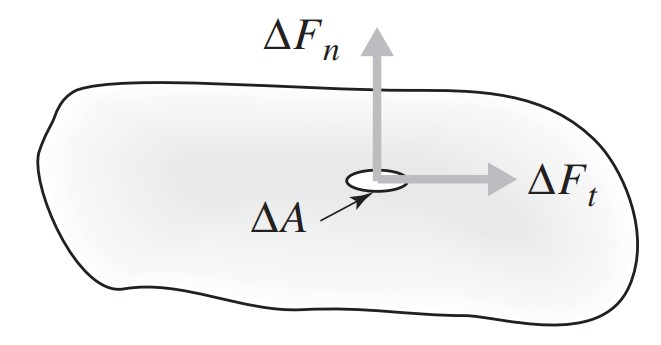
\includegraphics[width= .7\linewidth]{cortante2}
	\end{subfigure}
	\caption{Esfuerzo cortante}
\end{figure}

\end{document}